%!TEX root = ../../book_ML.tex
\chapter{Đối ngẫu}
\label{cha:duality}
\index{doi@đối ngẫu -- duality}
\index{duality -- đối ngẫu}
% \textbf{Trong bài viết này, chúng ta giả sử rằng các đạo hàm đều tồn tại.}

% \textbf{Bài viết này chủ yếu được dịch lại từ Chương 5 của cuốn \textit{Convex Optimization} trong tài liệu tham khảo.}

% \textit{Nếu bạn gặp khó khăn trong việc hiểu đạo hàm trong bài viết này, bạn được khuyến khích đọc \href{http://machinelearningcoban.com/math/#-dao-ham-cua-ham-nhieu-bien}{Đạo hàm của hàm nhiều biến}. Ngoài ra, các kiến thức trong \href{http://machinelearningcoban.com/2017/03/12/convexity/}{Bài 16} và \href{http://machinelearningcoban.com/2017/03/19/convexopt/}{Bài 17} là quan trọng để hiểu rõ hơn bài viết này.}


\section{Giới thiệu }
Trong Chương~\ref{cha:convexity} và Chương~\ref{cha:cvxopt}, chúng ta đã
thảo luận về tập lồi, hàm lồi và các bài toán tối ưu lồi. Trong chương này, chúng ta sẽ tiếp tục
tìm hiểu sâu hơn scác điều kiện về nghiệm của các bài toán tối ưu, cả
lồi và không lồi; \textit{bài toán đối ngẫu} ({dual problem}) và điều
kiện KKT.

% Trước tiên, chúng ta lại bắt đầu bằng những kỹ thuật đơn giản cho các bài toán cơ bản. Kỹ thuật này có lẽ các bạn đã từng nghe đến: Phương pháp nhân tử Lagrange (method of \href{https://en.wikipedia.org/wiki/Lagrange_multiplier}{Lagrange multipliers}). Đây là một phương pháp giúp tìm các điểm cực trị của hàm mục tiêu trên feasible set của bài toán.

% Nhắc lại rằng giá trị lớn nhất và nhỏ nhất (nếu có) của một hàm số $f_0(\mathbf{x})$ khả vi (và tập xác định là một \href{https://en.wikipedia.org/wiki/Open_set}{\textit{tập mở}}) đạt được tại một trong các điểm cực trị của nó. Và điều kiện cần để một điểm là điểm cực trị là đạo hàm của hàm số tại điểm này $f_0'(x) = 0$. Chú ý rằng một điểm thoả mãn $f_0'(\mathbf{x})$ = 0 thì được gọi là \textit{điểm dừng} hay \textit{stationary point}. Điểm cực trị là một điểm dừng nhưng không phải điểm dừng nào cũng là điểm cực trị. Ví dụ hàm $f(x) = x^3$ có $0$ là một điểm dừng nhưng không phải là điểm cực trị.

% Với hàm nhiều biến, ta cũng có thể áp dụng quan sát này. Tức chúng ta cần đi tìm nghiệm của phương trình đạo hàm \textit{theo mỗi biến} bằng 0. Tuy nhiên, đó là với các bài toán không ràng buộc (unconstrained optimization problems), với các bài toán có ràng buộc như chúng ta đã gặp trong Bài 17 thì sao?
\index{nhân tử Lagrange -- Lagrange multiplier}
\index{Lagrange multiplier -- nhân tử Lagrange}
Trước tiên chúng ta xét bài toán tối ưu chỉ có một phương trình ràng buộc:
\begin{equation}
\label{eqn:18_1constraint0}
\begin{aligned}
\mathbf{x}=& \arg\min_{\mathbf{x}} f_0(\mathbf{x}) \\\
\text{thoả mãn:}~& f_1(\mathbf{x}) = 0
\end{aligned}
\end{equation}
Bài toán này không nhất thiết là bài toán tối ưu lồi. Tức hàm mục tiêu
và hàm ràng buộc không nhất thiết phải lồi. Bài toán này có thể được giải bằng
phương pháp nhân tử Lagrange (xem Phụ Lục~\ref{apd:lagrange}). Cụ thể, xét hàm
số:
\begin{equation}
\label{eqn:simple_lagrange}
\mathcal{L}(\bx, \lambda) = f_0(\bx) + \lambda f_1(\bx)
\end{equation}
Hàm số
$\mathcal{L}(\mathbf{x}, \lambda)$ được gọi là \textit{hàm Lagrange}
(the Lagrangian) của bài toán tối ưu~\eqref{eqn:18_1constraint0}. Trong
hàm số này, chúng ta có thêm một biến  $\lambda$ được gọi là
\textit{nhân tử Lagrange} ({Lagrange multiplier}). Người ta đã chứng
minh được rằng, điểm tối ưu của bài toán
\eqref{eqn:18_1constraint0} thoả mãn điều kiện $\nabla_{\mathbf{x}, \lambda}
\mathcal{L}(\mathbf{x}, \lambda) = 0$. Tức là:
\begin{eqnarray}
\label{eqn:18_20}
\nabla_{\bx} \mathcal{L}(\bx, \lambda) = \nabla_{\mathbf{x}}f_0(\mathbf{x}) + \lambda \nabla_{\mathbf{x}} f_1(\mathbf{x}) &=& \bzero \\\
\label{eqn:18_30}
\nabla_{\lambda} \mathcal{L}(\bx, \lambda) = f_1(\mathbf{x}) & = & 0
\end{eqnarray}
Để ý rằng điều kiện thứ hai chính là phương trình ràng buộc trong bài toán
\eqref{eqn:18_1constraint0}.
Trong nhiều
trường hợp, việc giải hệ phương trình \eqref{eqn:18_20} - \eqref{eqn:18_30} đơn giản hơn việc trực tiếp đi tìm \textit{optimal value} của bài
toán \eqref{eqn:18_1constraint0}. Một số ví dụ về phương pháp nhân tử Lagrange
có thể được tìm thấy tại Phụ Lục~\ref{apd:lagrange}.

% Xét các ví dụ đơn giản sau đây.

% \subsection{Ví dụ}
% \textbf{Ví dụ 1:} Tìm giá trị lớn nhất và nhỏ nhất của hàm số $f_0(x, y) = x + y$ thoả mãn điều kiện $f_1(x, y) = x^2 + y^2 = 2$. Ta nhận thấy rằng đây không phải là một bài toán tối ưu lồi vì \textit{feasible set} $x^2 + y^2 = 2$ không phải là một tập lồi (nó chỉ là một đường tròn).

% \textbf{\textit{Lời giải:}}

% \textit{Lagrangian} của bài toán này là: $\mathcal{L}(x, y, \lambda) = x + y + \lambda(x^2 + y^2 - 2)$. Các điểm cực trị của hàm số Lagrange phải thoả mãn điều kiện:

% \begin{equation}
% \label{eqn:18_ex1}
% \nabla_{x, y, \lambda} \mathcal{L}(x, y, \lambda) = 0 \Leftrightarrow
% \left\{
% \begin{matrix}
%     1 + 2\lambda x &= 0 \\\
%     1 + 2\lambda y &= 0 \\\
%     x^2 + y^2 &=     2
% \end{matrix}
% \right.
% \end{equation}

% Từ hai phương trình đầu của \eqref{eqn:18_ex1} ta suy ra $x = y = \frac{-1}{2\lambda}$. Thay vào phương trình  ta sẽ có $\lambda^2 = \frac{1}{4} \Rightarrow \lambda = \pm \frac{1}{2}$. Vậy ta được 2 cặp nghiệm $(x, y) \in \{(1, 1), (-1, -1)\}$. Bằng cách thay các giá trị này vào hàm mục tiêu, ta tìm được giá trị nhỏ nhất và lớn nhất của hàm số cần tìm.

% \textbf{Ví dụ 2: Cross-entropy}. Trong \href{http://machinelearningcoban.com/2017/01/27/logisticregression/}{Chương 10} và \href{http://machinelearningcoban.com/2017/02/17/softmax/}{Chương 13}, chúng ta đã được biết đến hàm mất mát ở dạng \href{http://machinelearningcoban.com/2017/02/17/softmax/#-cross-entropy}{\textit{cross entropy}}. Chúng ta cũng đã biết rằng hàm cross entropy được dùng để đo sự giống nhau của hai phân phối xác suất với giá trị của hàm số này càng nhỏ thì hai xác suất càng gần nhau. Chúng ta cũng đã phát biểu rằng giá trị nhỏ nhất của hàm cross entopy đạt được khi từng gặp xác suất là giống nhau. Bây giờ, tôi xin phát biểu lại và chứng minh nhận định trên.

% Cho một phân bố xác xuất $\mathbf{p} = [p_1, p_2, \dots, p_n]^T$ với $p_i \in [0, 1]$ và $\sum_{i=1}^n p_i = 1$. Với một phân bố xác suất bất kỳ $\mathbf{q} = [q_1, q_2, \dots, q_n]$ và giả sử rằng $q_i \neq 0, \forall i$, hàm số cross entropy được định nghĩa là:
% \begin{equation*}
% f_0(\mathbf{q}) = -\sum_{i=1}^n p_i \log(q_i)
% \end{equation*}
% Hãy tìm $\mathbf{q}$ để hàm cross entropy đạt giá trị nhỏ nhất.

% Trong bài toán này, ta có ràng buộc là $\sum_{i=1}^n q_i = 1$. \textit{Lagrangian} của bài toán là:
% \begin{equation*}
% \mathcal{L}(q_1, q_2, \dots, q_n, \lambda) = -\sum_{i=1}^n p_i \log(q_i) + \lambda(\sum_{i=1}^n q_i - 1)
% \end{equation*}
% Ta cần giải hệ phương trình:

% \begin{equation*}
% \nabla_{q_1, \dots, q_n, \lambda} \mathcal{L}(q_1, \dots, q_n, \lambda) = 0 \Leftrightarrow
% \left\{
% \begin{matrix}
%    -\frac{p_i}{q_i} + \lambda = 0, ~~ i = 1, \dots, n\\\
%    q_1 + q_2 + \dots + q_n =1
% \end{matrix}
% \right.
% \end{equation*}

% Từ phương trình thứ nhất ta có $p_i = \lambda q_i$. Vậy nên: $ 1 = \sum_{i=1}^n p_i = \lambda\sum_{i=1}^n q_i = \lambda \Rightarrow \lambda = 1 \Rightarrow q_i = p_i, \forall i$.

% Qua đây, chúng ta đã hiểu rằng vì sao hàm số cross entropy được dùng để \textit{ép} hai xác suất \textit{gần nhau}.


\section{Hàm đối ngẫu Lagrange}
% \index{Lagrange!Lagrangian}
% \index{Lagrange!dual function}
\index{bài toán chính -- dual problem}
\index{dual problem -- bài toán chính}
\index{hàm số Lagrange -- Lagrangian}
\index{Lagrangian -- hàm số Lagrange}
\subsection{Hàm Lagrange của bài toán tối ưu}
Xét bài toán tối ưu tổng quát:
\begin{eqnarray}
\label{eqn:18_lagrangian}
\begin{aligned}
\mathbf{x}^* &= \arg\min_{\mathbf{x}} f_0(\mathbf{x}) \\
\text{thoả mãn:}~ & f_i(\mathbf{x}) \leq 0, ~~ i = 1, 2, \dots, m\\
& h_j(\mathbf{x}) = 0, ~~ j = 1, 2, \dots, p
\end{aligned}
\end{eqnarray}
với tập xác định $\mathcal{D} = \bigcap_{i=0}^m \dom f_i) \cap (\bigcap_{j=1}^p \dom
h_j$. Chú ý rằng, ở đây không có giả sử về tính chất lồi của hàm tối ưu
hay các hàm ràng buộc. Giả sử duy nhất là tập xác định $\mathcal{D} \neq
\emptyset$ (tập rỗng). Bài toán tối ưu này còn được gọi là \textit{bài toán chính} ({primal problem}).

Hàm số Lagrange cũng được xây dựng tương tự với mỗi nhân tử Lagrange cho một (bất) phương trình ràng buộc:
\begin{equation*}
\mathcal{L}(\mathbf{x}, \blambda, \bnu) = f_0(\mathbf{x}) + \sum_{i=1}^m \lambda_if_i(\mathbf{x}) + \sum_{j=1}^p \nu_j h_j(\mathbf{x}).
\end{equation*}
Trong đó, $\blambda = [\lambda_1, \lambda_2, \dots, \lambda_m]; \bnu = [\nu_1, \nu_2,
\dots, \nu_p]$ là các vector được gọi là \textit{biến đối ngẫu}
({dual variable}) hoặc \textit{vector nhân tử Lagrange}
({Lagrange multiplier vector}). Nếu biến chính $\mathbf{x} \in
\mathbb{R}^n$ thì tổng số biến của hàm số Lagrange là $n + m + p$.
\index{biến đối ngẫu -- dual variable}
\index{dual variable -- biến đối ngẫu}
% \index{vector nhân tử Lagrange -- Lagrange multiplier}
% (\textit{Thông thường, tôi dùng các chữ cái viết thường in đậm để biểu diễn một vector, trong trường hợp này tôi không bôi đậm được $\lambda$ và $\nu$ do hạn chế của LaTeX khi viết cùng markdown. Tôi lưu ý điều này để hạn chế nhầm lẫn cho bạn đọc})


\subsection{Hàm đối ngẫu Lagrange }
% \index{Lagrange/Lagrangian!dual functions}
\index{hàm đối ngẫu Lagrange -- the Lagrange dual function}
\index{the Lagrange dual function -- hàm đối ngẫu Lagrange}
\textit{Hàm đối ngẫu Lagrange} ({the Lagrange dual function}) của bài toán
tối ưu (viết gọn là \textit{hàm số đối ngẫu}) \eqref{eqn:18_lagrangian} là một
hàm của các biến đối ngẫu $\blambda$ và $\bnu$, được định nghĩa là infimum theo $\mathbf{x}$
của hàm Lagrange:
\begin{equation}
g(\blambda, \bnu) = \inf_{\mathbf{x} \in \mathcal{D}} \mathcal{L}(\mathbf{x},
\blambda, \bnu)\\\
= \inf_{\mathbf{x} \in \mathcal{D}}\left( f_0(\mathbf{x}) + \sum_{i=1}^m \lambda_if_i(\mathbf{x}) + \sum_{j=1}^p \nu_j h_j(\mathbf{x})\right)
\end{equation}
Nếu hàm Lagrange không bị chặn dưới, hàm đối ngẫu tại $\blambda, \bnu$ lấy giá trị $-\infty$.

\textit{Lưu ý}:
\begin{itemize}
\item $\inf$ được lấy trên miền $x \in \mathcal{D}$, tức tập xác định của
bài toán. Tập xác
định này khác với tập khả thi  --  là tập hợp các điểm thoả mãn các
ràng buộc.

\item Với mỗi $\mathbf{x}$, hàm số đối ngẫu là một hàm {affine}
của $(\blambda, \bnu)$, tức là một hàm vừa lồi, vừa lõm. {Hàm
đối ngẫu} chính là một {infimum} từng thành phần của (có thể vô hạn) các hàm
lõm, tức cũng là một hàm lõm. Như vậy, \textbf{hàm đối ngẫu của một bài toán
tối ưu bất kỳ là một hàm lõm, bất kể bài toán tối ưu đó có là bài toán tối ưu lồi hay không}. Nhắc lại rằng {supremum} từng thành phần của các hàm
lồi là một hàm lồi; và một hàm là lõm nếu hàm đối của nó là một hàm lồi (xem thêm
Mục~\ref{ssub:16_properties}).
\end{itemize}



\subsection{Chặn dưới của giá trị tối ưu }
Nếu $p^*$ là giá trị tối ưu của bài toán
\eqref{eqn:18_lagrangian} thì với các biến đối ngẫu $\lambda_i \geq 0, \forall
i$ và $\bnu$ {bất kỳ}, ta sẽ có
\begin{equation}
\label{eqn:18_10}
g(\blambda, \bnu) \leq p^*
\end{equation}
Tính chất này có thể được chứng minh như sau. Giả sử $\mathbf{x}_0$ là một
điểm khả thi bất kỳ của bài toán \eqref{eqn:18_lagrangian}, tức
thoả mãn các điều kiện ràng buộc $f_i(\mathbf{x}_0) \leq 0, \forall i = 1,
\dots, m; h_j(\mathbf{x}_0) = 0, \forall j = 1, \dots, p$, ta sẽ có
\begin{equation*}
\mathcal{L}(\mathbf{x}_0, \blambda, \bnu) = f_0(\bx_0) + \sum_{i=1}^m
\underbrace{\lambda_if_i(\mathbf{x}_0)}_{\leq 0}+ \sum_{j=1}^p \underbrace{\nu_j
h_j(\mathbf{x}_0)}_{= 0} \leq f_0(\mathbf{x}_0)
\end{equation*}
Vì điều này đúng với mọi điểm khả thi $\mathbf{x}_0$, ta có tính chất quan trọng sau đây:
\begin{equation*}
g(\blambda, \bnu) = \inf_{\mathbf{x} \in \mathcal{D}} \mathcal{L}(\mathbf{x}, \blambda, \bnu) \leq \mathcal{L}(\mathbf{x}_0, \blambda, \bnu) \leq f_0(\mathbf{x}_0).
\end{equation*}
Khi $\mathbf{x}_0 = \mathbf{x}^*$ (điểm tối ưu), $f_0(\bx_0) = p^*$, ta suy ra
bất đẳng thức \eqref{eqn:18_10}.
Bất đẳng thức quan trọng này chỉ ra rằng giá trị tối ưu của hàm mục tiêu trong
bài toán chính~\eqref{eqn:18_lagrangian} không nhỏ hơn giá trị lớn nhất của hàm
đối
ngẫu Lagrange $g(\blambda, \bnu)$.

\subsection{Ví dụ }

\textit{Ví dụ 1:} Xét bài toán tối ưu:
\begin{equation}
\begin{aligned}
x&= \arg\min_{x} x^2 + 10\sin(x) + 10 \\\
\text{thoả mãn:}~& (x-2)^2 \leq 4
\end{aligned}
\end{equation}
Trong bài toán này, tập xác định $\mathcal{D} = \mathbb{R}$ nhưng
tập khả thi là $0 \leq x \leq 4$. Đồ thị của hàm mục tiêu được minh
hoạ bởi đường nét đậm trong Hình~\ref{fig:18_dualitya}. Hàm số ràng buộc
$f_1(x) = (x-2)^2 - 4$ được biểu diễn bởi đường chấm gạch. Có thể nhận ra rằng giá trị tối ưu
của bài toán là điểm trên đồ thị có hoành độ bằng 0 (là
điểm nhỏ nhất trên đường nét đậm trong đoạn $[0, 4]$). Chú ý rằng hàm mục tiêu không phải là hàm lồi nên bài toán tối ưu cũng
không phải là lồi, mặc dù hàm bất phương trình ràng buộc $f_1(x)$ là lồi.

% \newpage
Hàm số Lagrange của bài toàn này có dạng
\begin{equation*}
\mathcal{L}(x, \lambda) = x^2 + 10\sin(x) +10+ \lambda((x-2)^2 - 4)
\end{equation*}
Các đường nét chấm trong Hình~\ref{fig:18_dualitya} là các đồ thị của hàm Lagrange ứng với
$\lambda$ khác nhau. Vùng bị chặn giữa hai đường thẳng đứng màu đen thể
hiện tập khả thi của bài toán.
% ******************************************************************************
\begin{figure}[t]
\begin{subfigure}{0.48\textwidth}
% 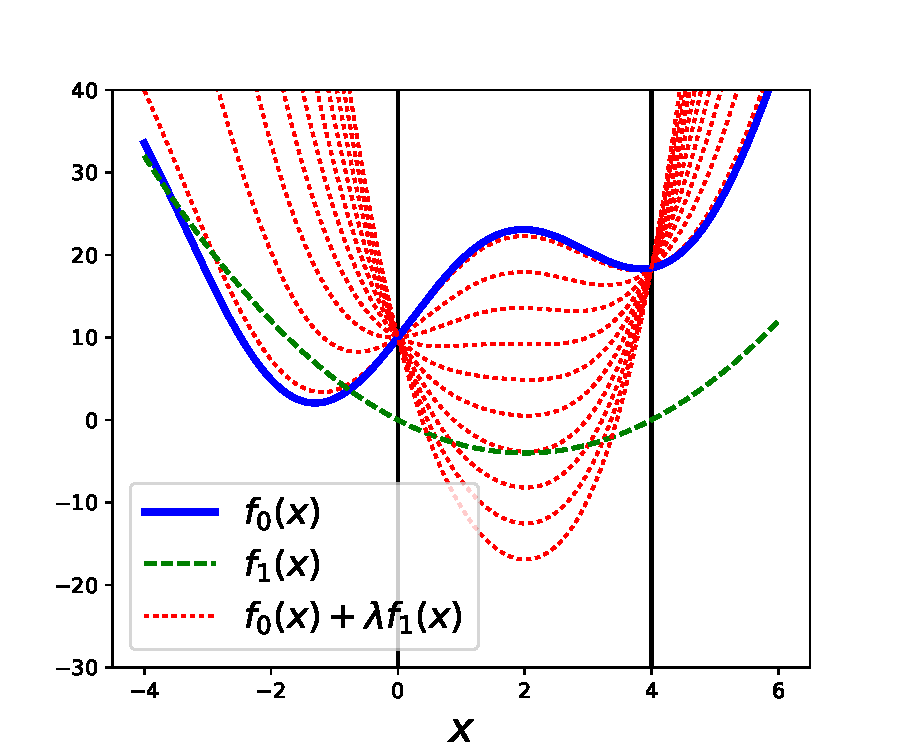
\includegraphics[width=0.95\linewidth]{Chapters/08_ConvexOptimization/18_duality/python/dual_func.pdf}
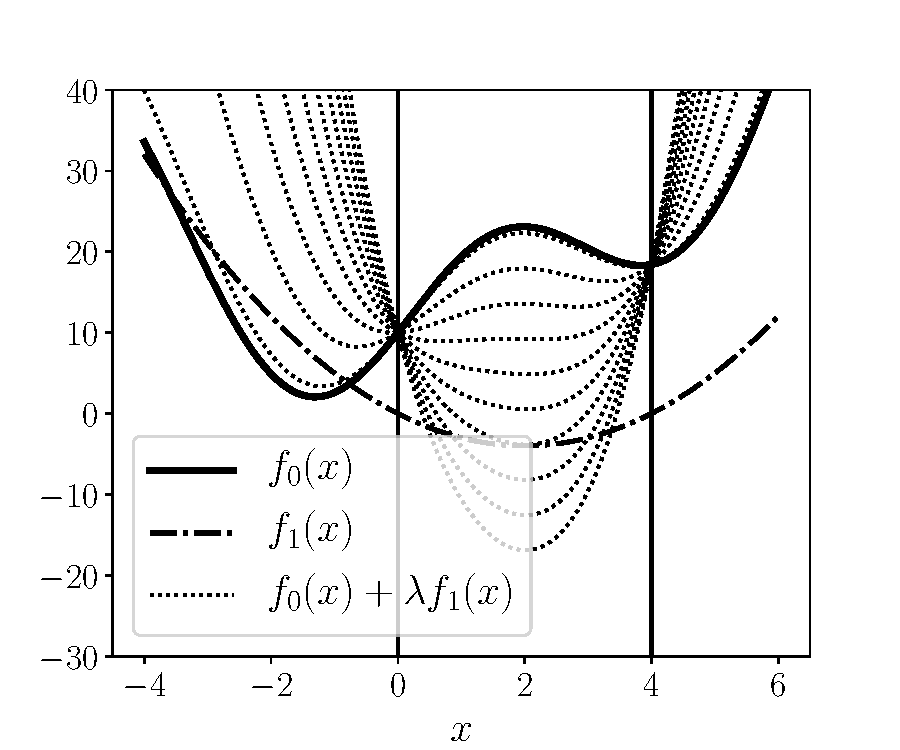
\includegraphics[width=0.95\linewidth]{ebookML_src/src/duality/dual_func.pdf}
\caption{}
\label{fig:18_dualitya}
\end{subfigure}
\begin{subfigure}{0.48\textwidth}
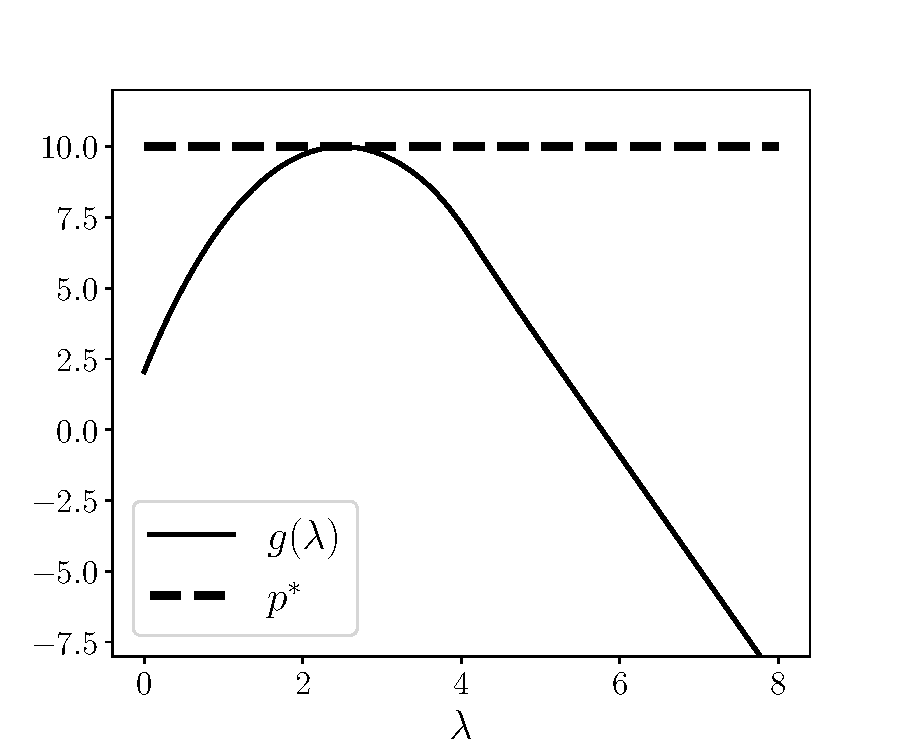
\includegraphics[width=0.95\linewidth]{ebookML_src/src/duality/dual_func2.pdf}
\caption{}
\label{fig:18_dualityb}
\end{subfigure}
\caption{Ví dụ về hàm số đối ngẫu. (a) Đường nét liền đậm thể hiện hàm mục
tiêu. Đường chấm gạch thể hiện hàm số ràng buộc. Các đường chấm chấm
thể hiện hàm Lagrange ứng với $\lambda$ khác nhau. (b)
Đường nét đứt nằm ngang thể hiện giá trị tối ưu của bài toán. Đường nét liền thể
hiện hàm số đối ngẫu. Với mọi $\lambda$, giá trị của hàm đối ngẫu nhỏ
hơn hoặc bằng giá trị tối ưu của bài toán chính.}
\label{fig:18_duality}
\end{figure}
% ******************************************************************************

Với mỗi $\lambda$, hàm số đối ngẫu được định nghĩa là:
\begin{equation*}
g(\lambda) = \inf_{x} \left(x^2 + 10\sin(x) + 10+ \lambda((x-2)^2 - 4) \right), ~~ \lambda \geq 0.
\end{equation*}
Từ Hình~\ref{fig:18_dualitya}, có thể thấy rằng với các $\lambda$ khác
nhau, hàm $g(\lambda)$ đạt giá trị nhỏ nhất tại điểm có hoành độ bằng 0 của
đường nét liền hoặc tại một điểm thấp hơn điểm đó. Trong Hình~\ref{fig:18_dualityb}, đường nét liền thể hiện đồ thị của hàm $g(\lambda)$, đường nét đứt thể hiện
giá trị tối ưu của bài toán tối ưu chính. Ta có thể thấy hai
điều:
\begin{itemize}
\item Đường nét liền luôn nằm phía dưới (hoặc có đoạn trùng) đường nét
đứt.

\item Hàm $g(\lambda)$ là một hàm lõm.
\end{itemize}

Mã nguồn cho Hình~\ref{fig:18_duality} có thể được tìm thấy tại
\url{https://goo.gl/jZiRCp}.

\textit{Ví dụ 2}:
Xét một bài toán quy hoạch tuyến tính:
\begin{eqnarray}
\begin{aligned}
x &= \arg \min_{\mathbf{x}}{\mathbf{c}^T\mathbf{x}} \\\
\text{thoả mãn:} ~ &\mathbf{Ax} = \mathbf{b} \\\
& \mathbf{x} \succeq 0
\end{aligned}
\end{eqnarray}
Hàm ràng buộc cuối cùng có thể được viết lại thành $f_i(\mathbf{x}) = -x_i, i = 1,
\dots, n$. Hàm Lagrange của bài toán này là:
\begin{equation*}
\mathcal{L}(\mathbf{x}, \blambda, \bnu) = \mathbf{c}^T\mathbf{x} - \sum_{i=1}^n \lambda_i x_i + \bnu^T(\mathbf{Ax} - \mathbf{b})  = -\mathbf{b}^T\bnu + (\mathbf{c} + \mathbf{A}^T\bnu - \blambda)^T\mathbf{x}
\end{equation*}
(đừng quên điều kiện $\blambda \succeq 0$). Hàm đối ngẫu là
\begin{eqnarray}
g(\blambda, \bnu) = \inf_{\mathbf{x}}\mathcal{L}(\mathbf{x}, \blambda, \bnu)
=  -\mathbf{b}^T\bnu + \inf_{\mathbf{x}} (\mathbf{c} + \mathbf{A}^T\bnu -
\blambda)^T\mathbf{x}
\end{eqnarray}
Nhận thấy rằng hàm tuyến tính $\mathbf{d}^T\mathbf{x}$ của $\mathbf{x}$ bị
chặn dưới khi vào chỉ khi $\mathbf{d} = 0$. Vì nếu có một phần tử $d_i$ của
$\mathbf{d}$ khác 0, chỉ cần chọn $x_i$ rất lớn và ngược dấu với $d_i$, ta sẽ
có một giá trị nhỏ tuỳ ý. Nói cách khác, $g(\blambda, \bnu) = -\infty$ trừ khi
$\mathbf{c} + \mathbf{A}^T\bnu - \blambda = 0$. Tóm lại,
\begin{eqnarray}
g(\blambda, \bnu) = \left\{
\begin{matrix}
-\mathbf{b}^T\bnu & ~\text{nếu}~  \mathbf{c}+ \mathbf{A}^T\bnu - \blambda
= 0\\\
-\infty &\text{o.w.}
\end{matrix} \right.
\end{eqnarray}
Trường hợp thứ hai khi $g(\blambda,\bnu) = -\infty$ chúng ta sẽ gặp rất nhiều
sau này. Trường hợp này không mấy thú vị vì hiển nhiên $g(\blambda, \bnu) \leq
p^*$. Với mục đích chính là đi tìm chặn dưới của $p^*$, ta chỉ cần quan tâm tới
các giá trị của $\blambda$ và $\bnu$ sao cho $g(\blambda, \bnu)$ càng lớn càng
tốt. Trong bài toán này, ta sẽ quan tâm tới $\blambda$ và $\bnu$ sao cho
$\mathbf{c}+ \mathbf{A}^T\bnu - \blambda = 0$.


\section{Bài toán đối ngẫu Lagrange}

% \index{Lagrange!dual problem}
Với mỗi cặp $(\blambda, \bnu)$, hàm đối ngẫu Lagrange cho chúng ta một chặn dưới
cho giá trị tối ưu $p^*$ của bài toán chính~\eqref{eqn:18_lagrangian}. Câu
hỏi đặt ra là: với cặp giá trị nào của $(\blambda, \bnu)$, chúng ta sẽ có một
chặn dưới tốt nhất của $p^*$? Nói cách khác, ta đi cần giải bài toán
\begin{equation}
\label{eqn:18_11}
\begin{aligned}
\blambda^*, \bnu^* &= \arg \max_{\blambda, \bnu} g(\blambda, \bnu)   \\\
\text{thoả mãn:}~ & \blambda \succeq 0
\end{aligned}
\end{equation}
Đây là một bài toán tối ưu lồi vì ta cần tối đa một hàm lõm trên tập khả thi lồi. Trong nhiều trường hợp,
lời giải cho bài toán~\eqref{eqn:18_11} có thể dễ tìm hơn  bài toán chính.

% \textit{Bài toán}
% Chú ý rằng, bài toán tối ưu này là
% convex bất primal problem~\eqref{eqn:18_lagrangian} có là convex hay không.
\index{bài toán đối ngẫu Lagrange -- Lagrange dual problem}
\index{Lagrange dual problem -- bài toán đối ngẫu Lagrange}
\index{tập khả thi đối ngẫu -- dual feasible set}
\index{dual feasible set -- tập khả thi đối ngẫu}
Bài toán tối ưu~\eqref{eqn:18_11} được gọi là \textit{bài toán đối ngẫu Lagrange}
({Lagrange dual problem}) (hoặc viết gọn là \textit{bài toán đối ngẫu}) ứng với bài toán
chính~\eqref{eqn:18_lagrangian}. Tập khả thi của bài toán đối ngẫu được gọi là \textit{tập khả thi đối ngẫu} (dual feasible set). Ràng buộc của bài toán đối ngẫu bao
gồm điều kiện $\blambda \succeq 0 $ và điều kiện ẩn $g(\blambda, \bnu) >
-\infty$ (điều kiện này được thêm vào vì ta chỉ quan tâm tới các $(\blambda,
\bnu)$ sao cho hàm mục tiêu của bài toán đối ngẫu càng lớn càng tốt). Nghiệm của
bài toán đối ngẫu~\eqref{eqn:18_11} ký hiệu bởi $(\blambda^*,
\bnu^*)$, được gọi là \textit{điểm tối ưu đối ngẫu} (dual optimal point).
\index{die@điểm tối ưu đối ngẫu -- dual optimal point}
\index{dual optimal point -- điểm tối ưu đối ngẫu}

Trong nhiều trường hợp, điều kiện ẩn $g(\blambda, \bnu) > -\infty$
cũng có thể được viết cụ thể. Quay lại với ví dụ phía trên, điệu kiện ẩn có thể
được viết thành $\mathbf{c}+ \mathbf{A}^T\bnu - \blambda = 0$. Đây là một hàm
affine. Vì vậy, khi có thêm ràng buộc này, ta vẫn thu được một bài toán lồi.

\subsection{Đối ngẫu yếu}
\index{doi@đối ngẫu yếu -- weak duality}
\index{weak duality -- đối ngẫu yếu}
Ký hiệu giá trị tối ưu của bài toán đối ngẫu \eqref{eqn:18_11} là $d^*$. Theo
\eqref{eqn:18_10}, ta đã biết $d^* \leq p^*$. Tính chất quan trọng này được
gọi là \textit{đối ngẫu yếu} (weak duality).
% \newpage
Ta quan sát thấy hai điều:
\begin{itemize}
\item Nếu giá trị tối ưu trong bài toán chính là $p^* = -\infty$, ta phải có $d^* = -\infty$. Điều này tương đương với việc bài toán đối ngẫu là bất khả thi (không có giá trị nào thỏa mãn các ràng buộc).

\item Nếu hàm mục tiêu trong bài toán đối ngẫu không bị chặn trên, nghĩa là $d^*
= +\infty$, ta phải có $p^* = +\infty$. Khi đó, bài toán chính là bất khả thi.
\end{itemize}

Giá trị $p^* - d^*$ được gọi là \textit{cách biệt đối ngẫu tối ưu} (optimal duality gap). Cách biệt này luôn là một số không âm.

Đôi khi có những bài toán tối ưu (lồi hoặc không) rất khó giải. Tuy nhiên, nếu tìm được $d^*$, ta có thể biết chặn dưới của bài toán chính. Việc tìm
$d^*$ thường đơn giản hơn vì bài toán đối ngẫu luôn luôn là lồi.


% \subsection{Strong duality và Slater's constraint qualification }
\subsection{Đối ngẫu mạnh và tiêu chuẩn ràng buộc Slater}
\label{ssec:slatter}
\index{doi@đối ngẫu mạnh -- strong duality}
\index{strong duality -- đối ngẫu mạnh}
\index{tiêu chuẩn ràng buộc Slater -- Slater's constraint qualification}
\index{Slater's constraint qualification -- tiêu chuẩn ràng buộc Slater}
Nếu đẳng thức $p^* = d^*$ thoả mãn, cách biệt đối ngẫu tối ưu bằng
không, ta nói rằng \textit{đối ngẫu mạnh} (strong duality) xảy ra. Lúc này, việc giải bài
toán đối ngẫu đã giúp tìm được {chính xác} giá trị tối ưu của bài toán gốc.

Thật không may, đối ngẫu mạnh không thường xuyên xảy ra trong các
bài toán tối ưu. Tuy nhiên, nếu bài toán chính là lồi, tức có dạng
\begin{equation}
\label{eqn:18_12}
\begin{aligned}
x &= \arg \min_{\mathbf{x}} f_0(\mathbf{x})   \\\
\text{thoả mãn:}~ & f_i(\mathbf{x}) \leq 0, i = 1, 2, \dots, m\\\
& \mathbf{Ax} = \mathbf{b}
\end{aligned}
\end{equation}
trong đó $f_0, f_1, \dots, f_m$ là các hàm lồi, chúng ta {thường}
(không luôn luôn) có đối ngẫu mạnh. Rất nhiều nghiên cứu đã thiết lập các điều kiện ngoài tính chất lồi để đối ngẫu mạnh xảy ra. Những điều kiện đó có tên là \textit{tiêu chuẩn ràng buộc} (constraint qualification).

\index{tiêu chuẩn ràng buộc -- constraint qualification}
\index{constraint qualification -- tiêu chuẩn ràng buộc}

Một trong các tiêu chuẩn ràng buộc phổ biến nhất là \textit{tiêu chuẩn ràng buộc Slater} (Slater's constraint qualification).

Trước khi thảo luận về tiêu chuẩn ràng buộc Slatter, chúng ta cần định nghĩa:
\begin{mydef}{Khả thi chặt}{nolable}
Một điểm khả thi của bài toán \eqref{eqn:18_12}
được gọi là  \textit{khả thi chặt} (stricly feasible) nếu:
\begin{equation*}
f_i(\mathbf{x}) < 0, ~i = 1, 2, \dots, m, ~~~ \mathbf{Ax} = \mathbf{b}
\end{equation*}
\end{mydef}
Khả thi chặt khác với khả thi ở việc dấu bằng trong các bất phương trình ràng buộc không xảy ra.

\begin{mytheo}{Tiêu chuẩn ràng buộc Slater}{slatter}
Nếu bài toàn chính là một bài toán tối ưu lồi và tồn tại một điểm khả thi chặt thì đối ngẫu mạnh xảy ra.
\end{mytheo}
Điều kiện khá đơn giản sẽ giúp ích cho nhiều bài toán tối ưu sau này.

\textit{Chú ý:}
\begin{itemize}
\item Đối ngẫu mạnh không thường xuyên xảy ra. Với các bài toán lồi,
điều này xảy ra {thường xuyên hơn}. Tồn tại những bài toán lồi mà đối ngẫu mạnh không đạt được.

\item Có những bài toán không lồi nhưngđối ngẫu mạnh vẫn xảy ra.
Bài toán tối ưu trong Hình~\ref{fig:18_duality} là một ví dụ.
\end{itemize}

\section{Các điều kiện tối ưu}
\index{die@điều kiện lỏng lẻo bù trừ -- complementary slackness}
\index{complementary slackness -- điều kiện lỏng lẻo bù trừ}
\subsection{Sự lỏng lẻo bù trừ}
Giả sử đối ngẫu mạnh xảy ra. Gọi $\mathbf{x}^*$ là một điểm
tối ưu của bài toán chính và $(\blambda^*, \bnu^*)$ là cặp điểm tối ưu của bài toán đối ngẫu. Ta có
\begin{eqnarray}
\label{eqn:18_113}
f_0(\mathbf{x}^*) &=& g(\blambda^*,\bnu^*) \\
\label{eqn:18_114}
&=& \inf_{\mathbf{x}} \left(f_0(\mathbf{x}) + \sum_{i=1}^m \lambda_i^* f_i(\mathbf{x}) + \sum_{j=1}^p \nu_j^* h_j(\mathbf{x})\right)\\
\label{eqn:18_115}
&\leq& f_0(\mathbf{x}^*) + \sum_{i=1}^m \lambda_i^* f_i(\mathbf{x}^*) + \sum_{j=1}^p \nu_j^* h_j(\mathbf{x}^*) \\
\label{eqn:18_116}
&\leq& f_0(\mathbf{x}^*)
\end{eqnarray}
Đẳng thức \eqref{eqn:18_113} xảy ra do đối ngẫu mạnh. Đẳng thức
\eqref{eqn:18_114} xảy ra do định nghĩa của hàm đối ngẫu. Bất đẳng
thức~\eqref{eqn:18_115} là hiển nhiên vì infimum của một hàm nhỏ hơn giá trị của
hàm đó tại bất kỳ điểm nào khác. Bất đẳng thức~\eqref{eqn:18_116} xảy ra vì
các ràng buộc $f_i(\mathbf{x}^*) \leq 0, \lambda_i \geq 0, i = 1, 2, \dots, m$
và $h_j(\mathbf{x}^*) = 0$. Từ đây có thể thấy rằng dấu đẳng thức
ở~\eqref{eqn:18_115} và~\eqref{eqn:18_116} phải đồng thời xảy ra. Ta lại có
thêm hai quan sát thú vị nữa:
\begin{itemize}
\item $\mathbf{x}^*$ là một điểm tối ưu của $g(\blambda^*, \bnu^*)$.

\item Thú vị hơn, $\displaystyle \sum_{i=1}^m \lambda_i^* f_i(\mathbf{x}^*)
= 0$. Vì $\lambda^*f_i(\bx^*) \leq 0$, ta phải có
$\lambda_i^*f_i(\mathbf{x}^*) = 0,~\forall i$.
Điều kiện này được gọi là \textit{điều kiện lỏng lẻo bù trừ} (complementary slackness). Từ đây ta có:
\begin{eqnarray}
\lambda_i^* > 0 &\Rightarrow& f_i(\mathbf{x}^*) = 0 \\\
f_i(\mathbf{x}^*) < 0 &\Rightarrow& \lambda_i^* = 0
\end{eqnarray}
Tức một trong hai giá trị này phải bằng 0.
\end{itemize}

\subsection{Các điều kiện tối ưu KKT}
\label{ssec:kkt}
\index{die@điều kiện KKT -- KKT condition}
\index{KKT condition -- điều kiện KKT}
Ta vẫn giả sử rằng các hàm đang xét có đạo hàm và bài toán tối ưu không nhất
thiết là lồi.


\textit{\textbf{Điều kiện KKT cho bài toán tối ưu (không nhất thiết lồi)}}

Giả sử đối ngẫu mạnh xảy ra. Gọi $\mathbf{x}^*$ và $(\blambda^*, \bnu^*)$ là mộ bộ điểm tối ưu chính và tối ưu đối ngẫu. Vì $\mathbf{x}^*$ tối ưu hàm khả vi $\mathcal{L}(\mathbf{x}, \blambda^*, \bnu^*)$, đạo hàm của hàm Lagrange tại $\mathbf{x}^*$ phải bằng 0.

Điều kiện Karush-Kuhn-Tucker (KKT) nói rằng $\mathbf{x}^*, \blambda^*, \bnu^*$
phải thoả mãn:
\begin{eqnarray}
f_i(\mathbf{x}^*) &\leq& 0, i = 1, 2, \dots, m \\\
h_j(\mathbf{x}^*) &=& 0, j = 1, 2, \dots, p \\\
\lambda_i^* &\geq& 0, i = 1, 2, \dots, m \\\
\lambda_i^*f_i(\mathbf{x}^*) &=& 0, i = 1, 2, \dots, m \\\
\nabla_{\bx} f_0(\mathbf{x}^*) + \sum_{i=1}^m \lambda_i^* \nabla_{\bx} f_i(\mathbf{x}^*) + \sum_{j=1}^p\nu_j^* \nabla_{\bx} h_j(\mathbf{x}^*) &=& 0
\end{eqnarray}
Đây là {điều kiện cần} để $\mathbf{x}^*, \blambda^*, \bnu^*$ là nghiệm
của bài toán chính và bài toán đối ngẫu. Hai điều kiện đầu chính là ràng buộc của bài toán chính. Điều kiện $\lambda_i^*f_i(\bx^*)$ là điều kiện lỏng lẻo bù trừ. Điều kiện cuối cùng là đạo hàm của hàm Lagrange theo $\bx^*$ bằng không.


\textit{\textbf{Điều kiện KKT cho bài toán lồi}}

Với bài toán lồi và đối ngẫu mạnh xảy ra, các điều kiện KKT vừa đề cập cũng là điều kiện đủ. Vậy với các bài toán tối ưu lồi có hàm mục tiêu và
hàm ràng buộc là khả vi, bất kỳ bộ $(\bx*, \blambda^*, \bnu^*)$ nào thoả mãn các
điều kiện KKT đều là điểm tối ưu của bài toán chính và bài toán đối ngẫu.


Các điều kiện KKT rất quan trọng trong tối ưu. Trong một vài trường hợp đặc biệt
(chúng ta sẽ thấy trong Phần~\ref{cha:svm}), việc giải hệ (bất) phương
trình các điều kiện KKT là khả thi. Rất nhiều thuật toán tối ưu được xây
dựng dựa trên việc giải hệ điều kiện KKT.

\textit{Ví dụ:} Xét bài toán quy hoạch toàn phương với ràng buộc phương trình:
\begin{eqnarray}
\nonumber
\mathbf{x} &=& \arg \min_{\mathbf{x}} \frac{1}{2}\mathbf{x}^T\mathbf{Px} + \mathbf{q}^T\mathbf{x} + r  \\\
\text{thoả mãn:}~ && \mathbf{Ax} = \mathbf{b}.
\end{eqnarray}
Trong đó $\mathbf{P}$ làm một ma trận nửa nửa xác định dương. Hàm số Lagrange của bài
toán này là
\begin{equation*}
\mathcal{L}(\mathbf{x}, \bnu) = \frac{1}{2}\mathbf{x}^T\mathbf{Px} + \mathbf{q}^T\mathbf{x} + r  + \bnu^T(\mathbf{Ax} - \mathbf{b})
\end{equation*}
Hệ điều kiện KKT:
\begin{eqnarray}
\mathbf{Ax}^* &=& \mathbf{b} \\\
\mathbf{P}\mathbf{x}^* + \mathbf{q} + \mathbf{A}^T\bnu^* &=& 0
\end{eqnarray}
Phương trình thứ hai chính là phương trình đạo hàm của hàm Lagrange tại
$\mathbf{x}^*$ bằng 0. Hệ phương trình này có thể được viết lại dưới dạng
\begin{equation*}
\bmt
\mathbf{P} & \mathbf{A}^T \\\
\mathbf{A} & \mathbf{0}
\emt
\bmt
\mathbf{x}^* \\\
\bnu^*
\emt
=
\bmt
-\mathbf{q} \\\
\mathbf{b}
\emt
\end{equation*}
Đây là một phương trình tuyến tính đơn giản.

\section{Tóm tắt}
\textit{Giả sử rằng các hàm số đều khả vi.}
\begin{itemize}
\item Các bài toán tối ưu với ràng buộc chỉ gồm phương trình có thể được giải
bằng phương pháp nhân tử Lagrange. Điều kiện cần để một điểm là nghiệm của bài toán tối ưu là nó
phải thỏa mãn đạo hàm của hàm Lagrange bằng không.

\item Với các bài toán tối ưu (không nhất thiết lồi) có thêm ràng buộc là bất phương trình, chúng ta có hàm Lagrange tổng quát và các biến đối ngẫu Lagrange
$\blambda, \bnu$. Với các giá trị $(\blambda, \bnu)$ cố định, ta có định
nghĩa về hàm đối ngẫu Lagrange
$g(\blambda, \bnu)$. Hàm số này là infimum của hàm Lagrange khi
$\mathbf{x}$ thay đổi trên tập xác định của bài toán.


\item $g(\blambda, \bnu) \leq p^*$ với mọi $(\blambda, \bnu)$.

\item Hàm đối ngẫu Lagrange là lõm bất kể bài toán tối ưu chính có lồi hay không.

\item Bài toán đi tìm giá trị lớn nhất của hàm đối ngẫu Lagrange với điều
kiện $\blambda \succeq 0$ được gọi là {bài toán đối ngẫu}. Đây là một bài toán tối ưu lồi bất kể bài toán chính có lồi hay không.

\item Gọi giá trị tối ưu của bài toán đối ngẫu là $d^*$, ta có $d^*
\leq p^*$. Đây được gọi là đối ngẫu yếu.

\item Đối ngẫu mạnh xảy ra khi $d^* = p^*$. Trong các bài toán lồi, đối ngẫu mạnh thường xảy ra nhiều hơn.

\item Nếu bài toán chính là lồi và tiêu chuẩn ràng buộc Slater thoả mãn thì đối ngẫu mạnh xảy ra.

\item Nếu bài toán chính là lồi và đối ngẫu mạnh xảy ra thì điểm tối ưu thoả mãn các điều kiện KKT (điều kiện cần và đủ).

\item Rất nhiều bài toán tối ưu được giải quyết thông qua các điều kiện KKT.

\end{itemize}

% \section{Kết luận }

% Trong ba bài 16, 17, 18, tôi đã giới thiệu \textit{sơ lược} về tập lồi, hàm
% lồi, bài toán lồi, và các điệu kiện tối ưu được xây dựng thông qua
% \textit{duality}. Ý định ban đầu của tôi là tránh phần này vì khá nhiều toán,
% tuy nhiên trong quá trình chuẩn bị cho bài Support Vector Machine, tôi nhận
% thấy rằng cần phải giải thích về Lagrangian - kỹ thuật được sử dụng rất nhiều
% trong Tối ưu. Thêm nữa, để giải thích về Lagrangian, tôi cần nói về các bài
% toán lồi. Chính vì vậy tôi thấy có trách nhiệm \textit{phải} viết về ba bài
% này.

% Trong loạt bài tiếp theo, chúng ta sẽ lại quay lại với các thuật toán Machine
% Learning với rất nhiều ví dụ, hình vẽ và code mẫu. Nếu bạn nào có cảm thấy
% hơi đuối sau ba bài tối ưu này thì cũng đừng lo, mọi chuyện rồi sẽ ổn cả
% thôi.


% \section{Tài liệu tham khảo}
% [1] \href{http://stanford.edu/~boyd/cvxbook/}{Convex Optimization} – Boyd and Vandenberghe, Cambridge University Press, 2004.

% [2] \href{https://en.wikipedia.org/wiki/Lagrange_multiplier}{Lagrange Multipliers - Wikipedia}.
